%this is a test latex file
\documentclass{article}
\usepackage{CJK}
\usepackage{graphicx}
\usepackage{float}
%\usepackage{epstopdf}
%\usepackage{hyperref}
\begin{document}
\begin{CJK}{UTF8}{gbsn}
	\title {This is a test latex file}
	\author {Hanhj}
	\date {}
	\maketitle
	\tableofcontents
	\begin{abstract}
	\indent this is abstract
	\end{abstract}
	\part{part 1}
	\section{section1}section1
		\par
	    This is a test tex file\\
	你好aaa

        \part{jfkdl}
        \label{part:jk}

        \section{section2}	
		this is second section2\\
		中文,Hello 
		\subsection{section2.1}
		this is second paragrath 2.1.this is inline math:$\sum_a^bx_i^2$。
		this is outline math :$$y=x^2$$
		\par 
		this is next paragrath
		\newline
		this is new line

	\part{2}
	\paragraph{paragraph1}this is paragrath1
	\par
	this is new line aaaaaaaaaaaaaaaaaaaaaaaaaaaaaaaaaaaaaaaaaaa\\
	bbbbbbbbbbbbbbbbbbbbbbbbbbbbbbbbbbbbbbbbbbbbbbbbbb\\
	ccccccccccccccccccccccccc.
	\par 
	this is new paragraph
	\paragraph{paragraph2}
	this is paragraph2
	\subparagraph{subparagraph}
	\par 
	demo instert a pic\\
	\begin{figure}[H]
	\centering
	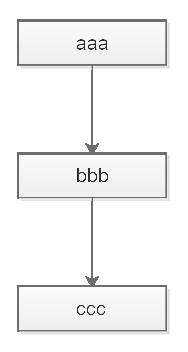
\includegraphics{test.eps}
	\caption{yes}
	\label{1}
	\end{figure}

	\begin{thebibliography}{123}
			\bibitem{JW1}aaa
			\bibitem{JW2}bbb
	\end{thebibliography}

\end{CJK}
\end{document}
